\documentclass{article}

\usepackage[utf8]{inputenc}
\usepackage[T1]{fontenc}
\usepackage{times}
\usepackage[cm]{fullpage}
\usepackage[parfill]{parskip}
\usepackage[xindy]{glossaries}
\usepackage{glossary-mcols}
\usepackage[french]{babel}
\usepackage{lmodern}
\usepackage{graphicx}
\usepackage[bottom]{footmisc}  % notes de bas de page réellement en bas de page

\graphicspath{{"Diagrams/"}}

\newglossary[glg]{glossary}{slm}{sbl}{Glossaire}
% si on ne précise pas le sort explicitement, il n'est pas content... Ça me gonfle donc je laisse comme ça pour l'instant...
% //~ TODO modifier le Sort des 2 derniers selon votre convenance

\newglossaryentry{Duel}{
    type=glossary,
    name={duel},
    description={Affrontement entre deux utilisateurs se solvant en la victoire de l'un des deux joueurs},
    sort=45
}

\newglossaryentry{Facultatif}{
    type=glossary,
    name={facultatif},
    description={Non-requis explicitement ou implicitement par le client mais qui pourra être implémenté par la suite},
    sort=65
}

\newglossaryentry{Deck}{
    type=glossary,
    name={deck},
    description={Paquet d'exactement 20 cartes de jeu ne comprenant pas plus de deux fois la même carte},
    sort=43
}

\newglossaryentry{Fosse}{
    type=glossary,
    name={fosse},
    description={\textit{Pseudo-lieu} du plateau où sont stockées les cartes ayant servi et étant arrivées en fin de vie},
    sort=67
}

\newglossaryentry{Lobby}{
    type=glossary,
    name={lobby},
    description={\textit{Pseudo} salle d'attente où les joueurs patientent le temps que le serveur leur désigne un adversaire},
    sort=125
}

\newglossaryentry{Invoquer}{
    type=glossary,
    name={invoquer},
    description={Utiliser une carte. Consiste à placer un monstre sur le terrain, attquer avec un monstre ou lancer un sort},
    sort=95
}
\newglossaryentry{Creature}{
    type=glossary,
    name={Creature},
    description={Une créature, (ou \textbf{Creature}) est une carte jouable sur le plateau. Elle dispose d'un certain montant de point de vie, d'un coût d'invocation, d'une
    valeur d'attaque et éventuellement d'un ou plusieurs effets, qu'il soit direct ou qu'il applique des contraintes à qui que ce soit.},
    sort=45
}
\newglossaryentry{Sort}{
    type=glossary,
    name={Sort},
    description={Un sort, (ou \textbf{Spell}) est une carte qui déclenche un effet à l'activation. Un sort ne dipose que d'un coût, et d'un ou plusieurs effets.},
    sort=45
},
\newglossaryentry{Pop}{
    type=glossary,
    name={Pop},
    description={Un pop est une action courante sur les piles informatique. Cette action consiste à enelever le sommet de la pile, et à souvent l'utiliser par la même occasion},
    sort=45
},
\newglossaryentry{Push}{
    type=glossary,
    name={Push},
    description={Un push est une action courante sur les piles informatique. Cette action consiste à ajouter un élément au dessus de la pile.},
    sort=45
}


\makeglossaries

\newglossarystyle{noIndex} {
	\renewenvironment{theglossary}
	{\vspace{-4em}
	\begin{longtable}{@{}p{0.15\textwidth}@{}p{0.85\textwidth}}}
	{\end{longtable}}
	\renewcommand*{\glossaryheader}{}
	\renewcommand*{\glsgroupheading}[1]{}
	\renewcommand*{\glossaryentryfield}[5]{\textbf{\glstarget{##1}{##2}} & ##3. \\}
}

\newglossarystyle{Index} {
	\renewenvironment{theglossary}
	{\vspace{-4em}
	\begin{longtable}{@{}p{0.15\textwidth}@{}p{0.85\textwidth}}}
	{\end{longtable}}
	\renewcommand*{\glossaryheader}{}
	\renewcommand*{\glsgroupheading}[1]{}
	\renewcommand*{\glossaryentryfield}[5]{\textbf{\glstarget{##1}{##2}} & ##5 \\}
}

\begin{document}

\pagenumbering{Roman}

\begin{titlepage}

\newcommand{\HRule}{\rule{\linewidth}{0.5mm}} % Defines a new command for the horizontal lines

\center % Center everything on the page

%----------------------------------------------------------------------------------------
%	HEADING SECTIONS
%----------------------------------------------------------------------------------------

\textsc{\LARGE Université libre de Bruxelles}\\[1.5cm]
\textsc{\Large INFO-F-209}\\[0.5cm]
\textsc{\large Projet d'année 2}\\[0.5cm]

%----------------------------------------------------------------------------------------
%	TITLE SECTION
%----------------------------------------------------------------------------------------

\HRule \\[0.4cm]
{ \huge \bfseries Software Requirement Document : Wizard Poker \\ Groupe 5}\\[0.4cm]
\HRule \\[1.5cm]

%----------------------------------------------------------------------------------------
%	AUTHOR SECTION
%----------------------------------------------------------------------------------------

\Large \emph{Auteurs :}\\
Baudoux Nicolas, Berrewaerts Jonathan, Gueniffrey Stanislas,  Muranovic Allan, Petit Robin, Reynouard Alexis et Verhelst Théo

%----------------------------------------------------------------------------------------
%	DATE SECTION
%----------------------------------------------------------------------------------------

{\large \today}\\[2cm]

%----------------------------------------------------------------------------------------
%	LOGO SECTION
%----------------------------------------------------------------------------------------

\includegraphics{ULB.png}\\[1cm]

%----------------------------------------------------------------------------------------

\vfill

\end{titlepage}


\tableofcontents
\newpage
\pagenumbering{arabic}

\section{Introduction}
	\subsection{But du projet}
		L'objectif visé par ce projet d'année de BA2 en sciences informatiques est la réalisation d'une application client-serveur en C/C++. L'application visée est
		un jeu de carte (appelé \textit{Wizard Poker}) au tour par tour et multijoueurs en réseau. Elle est destinée à tous types de public. Elle est également
		\textit{open source}, libre de droit et à but non commercial : c'est un projet académique.

		Pour ce faire, notre équipe, composée de sept personnes, dispose de trois phases de développement qui dureront approximativement 4 semaines chacune :
		\begin{itemize}
			\item la première portera uniquement sur la création du squelette respectant toutes les demandes effectuées par les client ;
			\item la deuxième phase concernera l'implémentation en console uniquement ;
			\item et enfin la troisième ajoutera l'interface graphique.
		\end{itemize}

		\subsubsection{Description du Wizard Poker}
			Le Wizard Poker est un jeu de cartes dans lequel deux joueurs s'affrontent en \gls{duel} au tour par tour. Chaque joueur a son propre \gls{deck}
			choisi parmi sa collection de cartes. Au début de chaque duel, les deux joueurs ont le même nombre de points de vie (à savoir 20) et piochent 5
			cartes de leur \gls{deck}.Le premier joueur sera choisi aléatoirement par le serveur. Ensuite, tout à tour, les joueurs pourront utiliser leurs cartes, qu'elles soient un \gls{Sort} ou une
			\gls{Creature} tant que leur coût d'utilisation/d'invocation/, ne dépasse pas l'énergie disponible du joueur. ( Le joueur gagne un point d'énergie supplémentaire par tour jusqu'à atteindre son maximum de 10.)
			Les cartes peuvent attaquer soit l'adversaire directmeent, soit une , soit une \gls{Creature} adverse. Ou encore avoir un ou plusieurs effets \textit{spéciaux}\footnote{Par exemple : \gls{invoquer} une carte au hasard, redonner de la vie, augmenter l'attaque, etc.}. Lorsqu'une carte
			arrive à la fin de sa période d'existence (points de vie de la carte arrivés à 0, sort détruisant ladite carte, effet terminé, etc.), elle est
			défaussée, c'est-à-dire qu'elle est envoyée dans la \gls{fosse}.
			Lorsqu'une carte est dans la \gls{fosse} (également appelé cimetière), elle
			peut éventuellement être réutilisée à l'aide de sorts particuliers par exemple. Une carte défaussée n'est pas perdue, elle reste propriété du joueur :
			à la fin de la partie, les joueurs ont les mêmes cartes qu'au début de la partie si ce n'est que le gagnant a reçu une carte supplémentaire
			suite à sa victoire. La partie s'arrête lorsqu'un des deux joueurs a un nombre inférieur ou égal à 0 points de vie ou a passé 10 tours sans carte en main.

			\begin{center}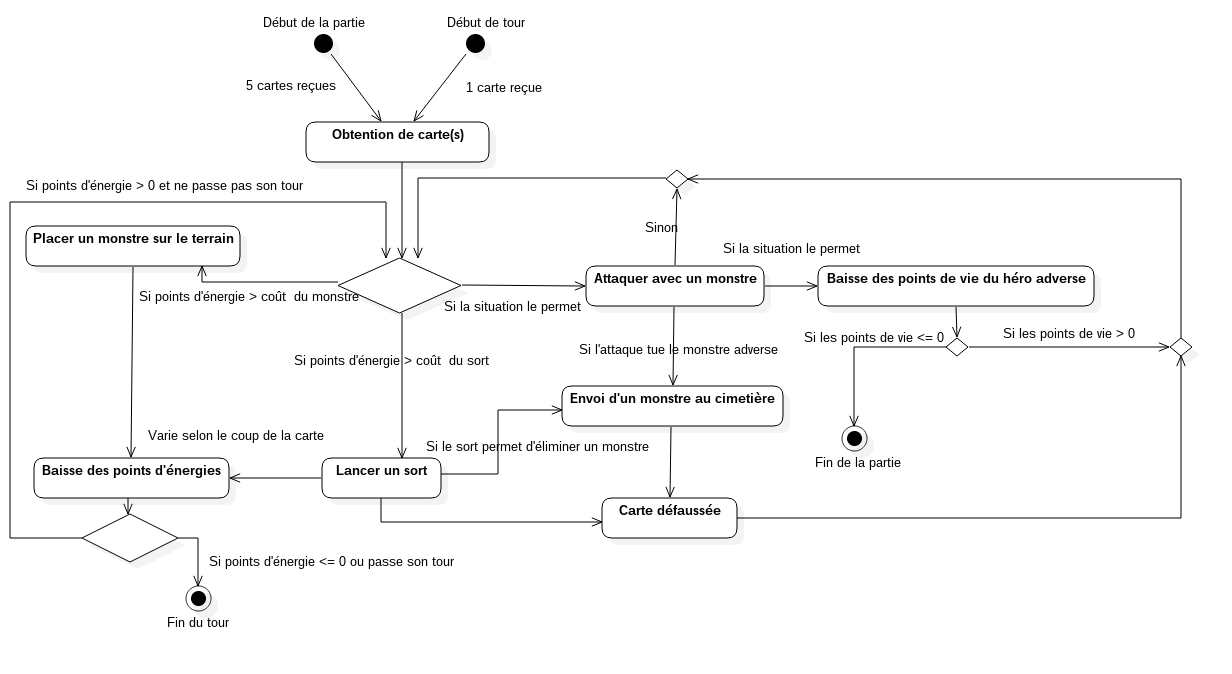
\includegraphics[scale=0.45]{Activity1_Gameplay.png}\end{center}

	\subsection{Glossaire}  % doit s'agrandir avec le temps (automatiquement)
		\printglossary[type=glossary, style=noIndex, title=]

	\subsection{Historique}
		\begin{itemize}
			\item[11/12/2015] Réunion (équipe complète) ;
			\item[11/12/2015] Squelette du SRD (équipe SRD) ;
			\item[15/12/2015] Création des diagrammes UML (équipe UML) ;
			\item[15/12/2015] Rédaction de la version propre du SRD (Robin).
			\item[31/01/2016] -> [26/02/2016] Développement du projet (en console uniquement).
			\item[25/02/2016]  Mise à jour du SRD (Allan).
		\end{itemize}

\newpage

\section{Besoins de l'utilisateur}
	L'utilisateur de l'application, à savoir le joueur, a un certain nombre de besoins. Ces derniers doivent être satisfaits afin de garantir un confort d'utilisation
	maximal. En utilisant l'application, le joueur \textbf{doit} avoir la possibilité de :

	\begin{itemize}
		\item créer un compte utilisateur ;
		\item créer un \gls{deck} ou en modifier un pré-existant ;
		\item consulter les cartes dont il dispose ;
		\item consulter les \glspl{deck} dont il dispose ;
		\item ajouter un joueur existant en ami ;
		\item discuter avec un ami ;
		\item \textbf{\gls{facultatif} :} discuter avec plusieurs amis simultanément ;
		\item affronter un adversaire aléatoire ;
		\item défier un joueur de sa liste d'amis ;
		\item consulter le classement des joueurs.
	\end{itemize}

	\subsection{Exigences fonctionnelles}
		\subsubsection{Possibilités d'actions de l'utilisateur}
			\begin{center}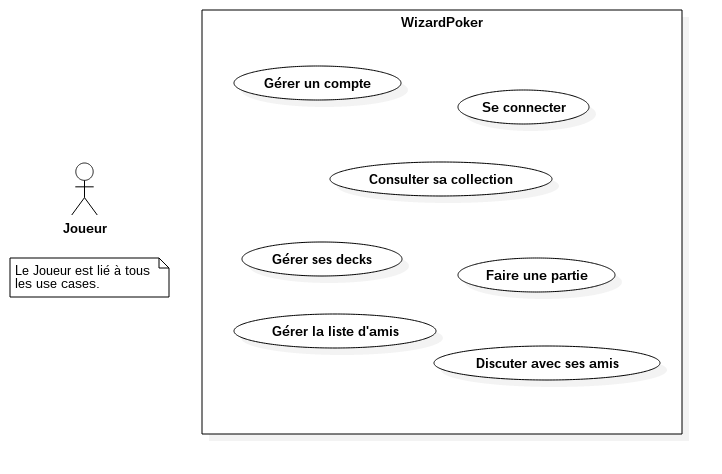
\includegraphics[scale=0.5]{UseCase1_Main.png}\end{center}
			\begin{itemize}
				% \TODO: remplacer Gérer un compte par Créer un compte dans UseCase1_Main.png
				\item \textbf{Créer un compte}
				\begin{description}
					\item[Description] Un utilisateur doit créer un compte pour pouvoir accéder à l'application.
					\item[Pré-condition] Aucune.
					\item[Post-condition] Un compte est crée, le nom d'utilisateur correspondant est unique.\\
				\end{description}

				\item \textbf{Se connecter}
				\begin{description}
					\item[Description] Un utilisateur doit se connecter avec un compte pour pouvoir acceder à l'application
					\item[Pré-condition] L'utilisateur n'est pas déjà connecté, le compte utilisé est existant est n'est pas déjà connecté.
					\item[Post-condition] L'utilisateur est connecté.\\
				\end{description}

				\item \textbf{Consulter sa collection}
				\begin{description}
					\item[Description] Un utilisateur peut voir la collection de cartes qu'il a acquises.
					\item[Pré-condition] Aucune.
					\item[Post-condition] L'utilisateur a pris connaissance sa collection de carte.\\
				\end{description}

				\item \textbf{Consulter sa collection}
				\begin{description}
					\item[Description] Un utilisateur peut voir la collection de cartes qu'il a acquises.
					\item[Pré-condition] Aucune.
					\item[Post-condition] L'utilisateur a pris connaissance sa collection de carte.\\
				\end{description}

				\item \textbf{Faire une partie}
				\begin{description}
					\item[Description] Un utilisateur peut jouer une partie.
					\item[Pré-condition] L'utilisateur a un deck actif.
					\item[Post-condition] Si l'utilisateur a gagné la partie, une carte est ajoutée à sa collection.
					Ses statistiques (parties gagnées / parties perdues) sont mises à jour.\\
				\end{description}

				\item \textbf{Discuter avec ses amis}
				\begin{description}
					\item[Description] Un utilisateur peut entamer une conversation avec d'autres joueurs, s'ils sont dans sa liste d'amis.
					\item[Pré-condition] L'utilisateur a au moins un ami, et l'ami
					\item[Post-condition] L'utilisateur\\
				\end{description}
			\end{itemize}

		\subsubsection{Création d'un compte}
			\begin{center}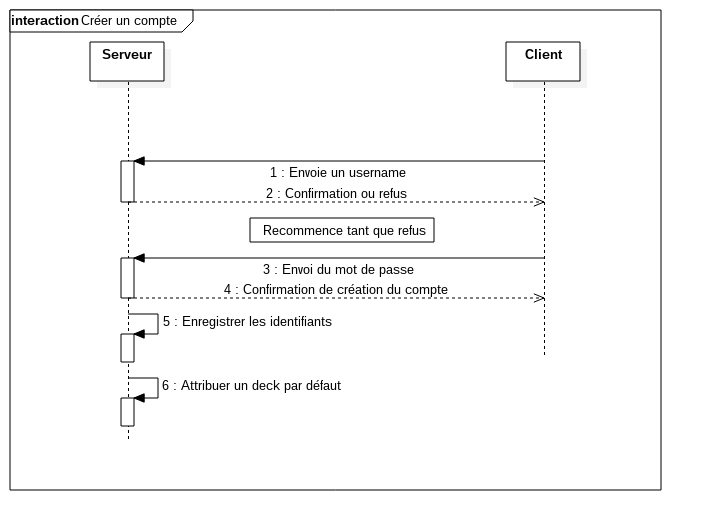
\includegraphics[scale=0.6]{Collaboration1_SignIn.png}\end{center}

			\begin{description}
				\item[Description] L'utilisateur peut créer un compte à l'aide d'un identifiant unique (son pseudo) et d'un mot de passe associé.
				\item[Pré-condition] L'utilisateur doit être connecté au serveur.
				\item[Post-condition] Soit la demande est acceptée (identifiant admissible), soit la demande est rejetée (identifiant non-admissible ou déjà utilisé).
			\end{description}

		\subsubsection{Gestion des \glspl{deck}}
			\begin{center}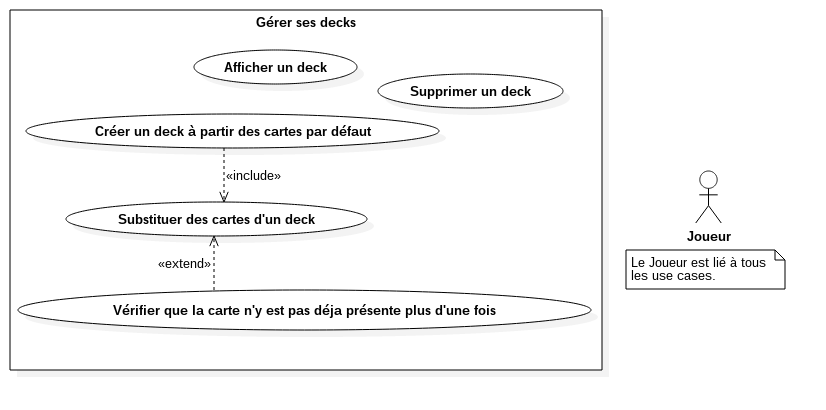
\includegraphics[scale=0.5]{Model1_DecksManagement.png}\end{center}
			\begin{itemize}
				\item \textbf{Supprimer un deck}
				\begin{description}
					\item[Description] Suppression d'un deck.
					\item[Pré-condition] La liste des decks n'est pas vide.
					\item[Post-condition] Il y a un deck en moins dans la liste des decks.\\
				\end{description}

				\item \textbf{Afficher un deck}
				\begin{description}
					\item[Description] Affichage d'un deck.
					\item[Pré-condition] La liste des decks n'est pas vide.
					\item[Post-condition] L'utilisateur a pris connaissance du contenu d'un deck.\\
				\end{description}

				\item \textbf{Créer un deck par défaut}
				\begin{description}
					\item[Description] Pour créer un nouveau deck, le deck par défaut est ajouté.
					\item[Pré-condition] Aucune.
					\item[Post-condition] Il y a un deck en plus dans la liste des decks.\\
				\end{description}

				\item \textbf{Changer les cartes d'un deck}
				\begin{description}
					\item[Description] Pour modifier un deck, il faut changer une par une les cartes qui le composent.
					\item[Pré-condition] La liste des decks n'est pas vide.
					\item[Post-condition] Un des decks la liste des decks a été modifié.\\
				\end{description}
			\end{itemize}
			Le fonctionnement de la création d'un nouveau deck nécessite peut-être quelques explications
			supplémentaire. Le use case "Créer un deck" commence par ajouter dans la liste des decks
			une copie du deck par défaut (celui donné à la création du compte). Ensuite l'utilisateur
			est redirigé vers le use case "Changer les cartes d'un deck", qui permet de remplacer
			une par une les cartes d'un deck. Ainsi, avec une grande modularité et peu de code,
			donné la possibilité de créer un tout nouveau deck sans devoir recoder une partie
			de l'interface qui modifie un deck.

		\subsubsection{Début de partie}
			\begin{center}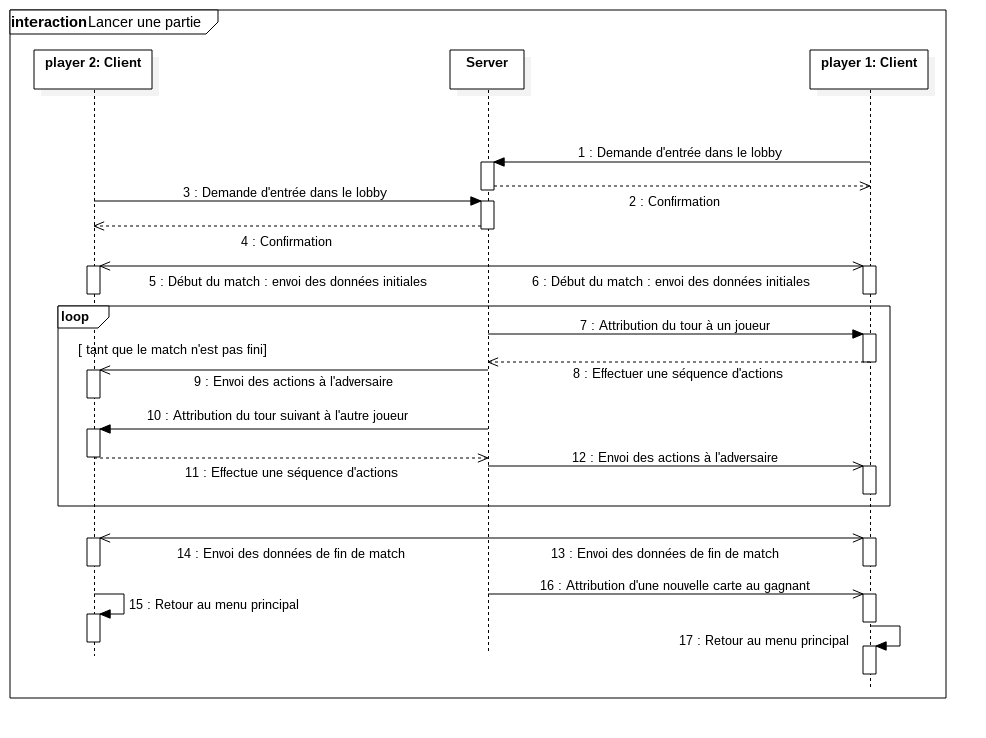
\includegraphics[scale=0.45]{Collaboration2_StartDuel.png}\end{center}

			\begin{description}
				\item[Description] Un joueur connecté peut défier un ami ou demander un duel contre un adversaire aléatoire.
				\item[Pré-condition] Chaque utilisateur doit être identifié et connecté à son compte.
				\item[Post-condition] Un joueur aura perdu, l'autre aura gagné\footnote{Le gagnant reçoit une carte aléatoire à ajouter à son \gls{deck}.}.
			\end{description}

		\subsubsection{Détail d'un tour}
			\begin{center}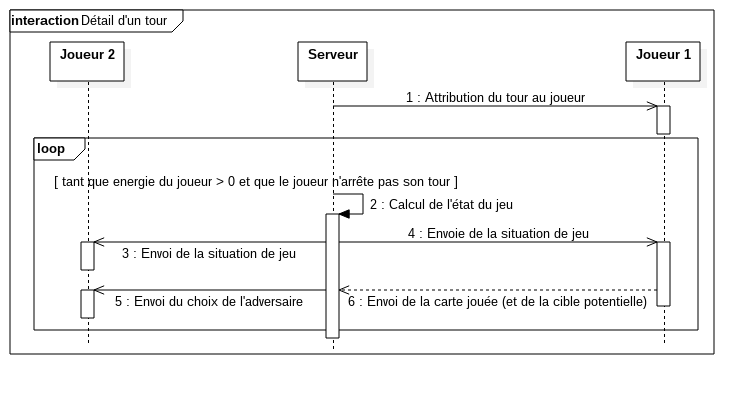
\includegraphics[scale=0.6]{Collaboration3_RoundDetails.png}\end{center}

	\subsection{Exigences non-fonctionnelles}
		L'application \textbf{doit} tourner sur Linux Debian (salles 008 et 009 du NO.4) et fonctionner en réseau (\textit{a priori} avec clients
		et serveurs sur des machines séparées).

		De plus, l'utilisateur \textbf{doit} pouvoir discuter par messages à n'importe quel moment de l'exécution de l'application : tant pendant
		qu'il gère ses amis, ses cartes ou pendant qu'il est en \gls{duel}. Ces discutions ne peuvent se faire avec un joueur
		n'étant pas ami de l'utilisateur.

	\subsection{Exigences de domaine}
		Les exigences implicites au domaine du jeu sont les suivante et sont \textbf{\glslink{facultatif}{facultatives}} :

		\begin{itemize}
			\item l'application doit être accessible à tout utilisateur potentiel ;
			\item l'application doit être \textit{amusante} donc équilibrée ;
			\item empêcher la triche dans la mesure du possible.
		\end{itemize}

\newpage

\section{Besoins du système}
	\subsection{Exigences fonctionnelles}
		Dans un premier temps, l'application \textbf{doit} tourner en ligne de commande et \textbf{doit}, dans un second temps adopter une interface
		graphique. De plus, l'application \textbf{doit} être développée en C++.

	\subsection{Exigences non-fonctionnelles}
		Le système \textbf{doit} être maintenable et pensé dans l'optique d'une future adaptation avec interface graphique.

	\subsection{Design et fonctionnement du système}
		La structure du programme est résumée dans le diagramme de classe ci-dessous. Chaque élément sera développé par après.
		\begin{center}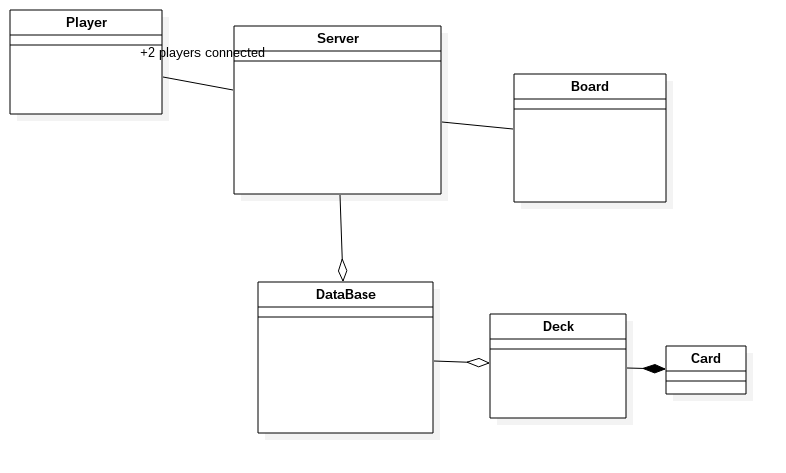
\includegraphics[scale=0.5]{Global.png}\end{center}

		Nous pouvons constater que le client (Player) se connecte au serveur qui, lui, gère les parties (le tableau de jeu) ainsi que la base de donnée et tout ce dont cette dernière comprend.

		\newpage
		\subsection{Diagramme de classe du \gls{deck} et des cartes}
		\begin{center}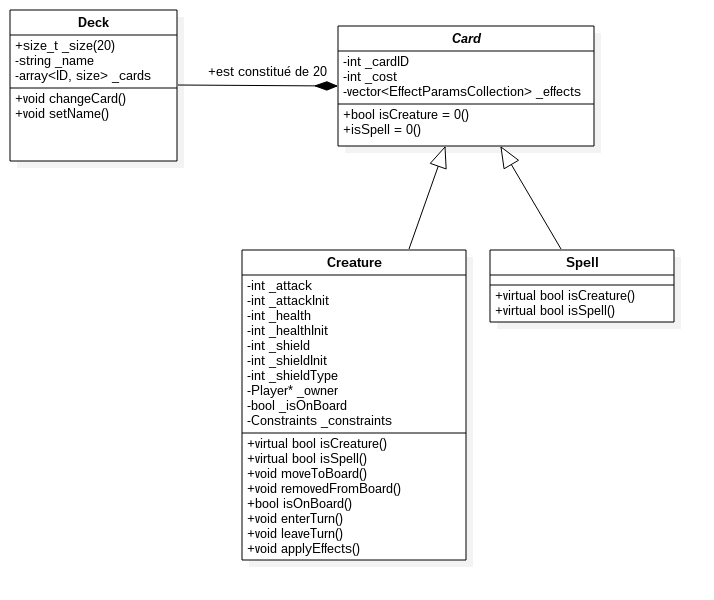
\includegraphics[scale=0.5]{deck.png}\end{center}
			Comme indiqué sur ce diagramme, un \gls{deck} est composé de cartes, 20 pour être précis. Les cartes sont soit des \gls{Creature}
			soit des \gls{Sort} et on ne peut posséder que maximum 2 exemplaire d'une même carte au sein d'un même \gls{deck}.
			A savoir également que les \gls{deck} sont indépendants, il est donc possible de posséder uniquement 2x la même carte,
			mais avoir plusieurs \gls{deck} qui possèdent 1 ou 2x cette carte.

			L'application des effets est simple : chaque effet est un effet direct, que ce soit infliger X points de dégats, comme soigner un allié ou encore interdire le joueur adverse de jouer pendant Y tours.
			Un effet plus complexe est également un effet direct, seulement, il va modifier la liste de contraintes de la partie et c'est cette liste qui va permettre d'appliquer des effets sur la durée, ou en respectant bien certaines conditions (applique tel effet tant que tel créature est en vie par exemple).

		\newpage
		\subsection{Diagramme de classe du serveur et de sa base de données}
		\begin{center}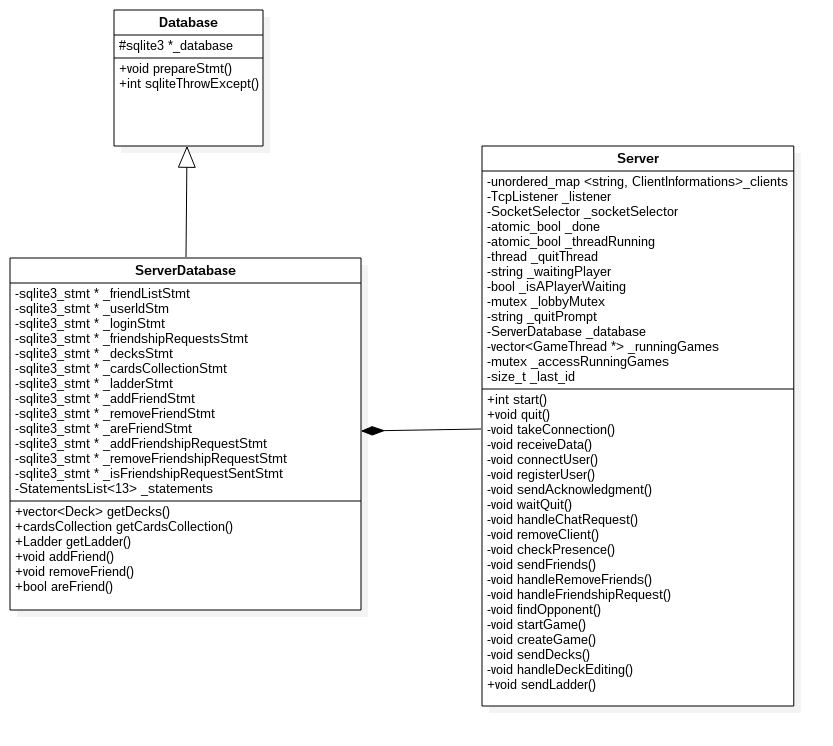
\includegraphics[scale=0.5]{Server.png}\end{center}
			Ici, la structure est un peu plus complexe : Le serveur est composé d'une base de donnée en SQL qui est héritée par 
			une base de donnée utilisable par l'application serveur (en c++ cette fois).

			C'est ce serveur qui va naturellement tout gérer, des parties, jusqu'aux requêtes d'amis en passant
			par la gestion/modification des \gls{deck}/de compte. Tout sera stocké de son côté dans la base de données.
			Le client ne possedera aucune données, il est obligé de passer par les serveur quel que soit son intention.

		\newpage
		\subsection{Diagramme des classes intervenant dans une partie (simplifié)}
		\begin{center}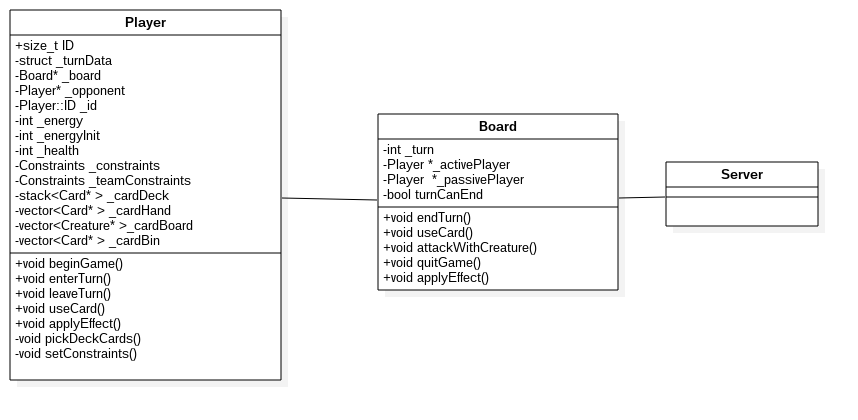
\includegraphics[scale=0.5]{Game.png}\end{center}
			Il est à noter que c'est un diagramme de classe, et non d'activités, il regroupe juste les plus grosses classes intervenant dans la partie,
			et non pas leur lien/fonctionnement entre elles.
			Pour qu'une partie puisse avoir lieu, il nous faut 2 joueurs connecté au serveur qui s'occupera lui-même de modifier le plateau de jeu.
			
	Toutes les méthodes servant à une expérience de jeu optimal sont implémentées, mais en console.
	L'interface graphique arrive à la prochaine étape du développement de ce projet, tout ce qui gère le fonctionnement du jeu est néanmoins présent.

\newpage

\section{Index}
		\printglossary[type=glossary, style=Index, title=]

\end{document}
